\documentclass[hyperref=colorlinks]{beamer}
\mode<presentation>
\usetheme{iclpt}
\setbeamertemplate{navigation symbols}{}
\setbeamertemplate{headline}{
\begin{beamercolorbox}[leftskip=.2cm,rightskip=.2cm,topskip=.2cm,ht=1.1cm,dp=0.1cm,wd=\textwidth]{institute in head/foot}
  
\includegraphics[height=1cm]{icl.pdf}
  \hfill
  
\includegraphics[height=1cm]{../Pics/CMS-Color.pdf}
\end{beamercolorbox}
}
\setbeamertemplate{footline}{
\begin{beamercolorbox}[ht=.55cm,dp=0.4cm,wd=\textwidth,leftskip=.3cm]{author in head/foot}%
  \begin{minipage}[c]{5cm}%
    \usebeamerfont{author in head/foot}
    \insertshortauthor 
    \insertshorttitle
    \end{minipage}\hfill%
  \insertframenumber{} / \pageref{lastframe}
  \hfill
  \begin{minipage}{6cm}
    \hfill
  \end{minipage}
\end{beamercolorbox}%
}

\usepackage{color}
\usepackage{tabularx,colortbl}
\usepackage{graphicx}
\usepackage{pdfpages}
\usepackage{feynmp}
\DeclareGraphicsRule{*}{mps}{*}{}

\title{\vspace{-0.2cm} Status of the VBF Higgs to Invisible Analysis}
\subtitle{AN-12-403,PAS-HIG-13-013 \vspace{-0.7cm}}
\author[P. Dunne]{ D.Colling, \underline{P. Dunne}, A. Magnan, A. Nikitenko, J. Pela with \\ R. Aggleton, J. Brooke: Bristol \\ C.Asawangtrakuldee, Q.Li: Peking \\ P. Srimanobhas: Chulalongkorn \\ S. Kumar, K. Mazumdar: Mumbai}
\titlegraphic{
  \vspace{-0.7cm}
\begin{fmfgraph*}(100,70)
        \fmfleft{i1,i2}
        \fmfright{o1,o2,o3}
        \fmf{fermion}{i1,v1,o1}
        \fmf{fermion}{i2,v2,o3}
        \fmf{phantom,tension=4/5}{v1,v2}
        \fmffreeze
        \fmf{photon,label=$W,,Z$}{v1,v3}
        \fmf{photon,label=$W,,Z$}{v2,v3}
        \fmf{dashes}{v3,o2}
        \fmflabel{$q$}{i1}
        \fmflabel{$q$}{i2}
        \fmflabel{$q$}{o1}
        \fmflabel{$q$}{o3}
        \fmflabel{$H$}{o2}
      \end{fmfgraph*}
}
\date{}
\begin{document}
\begin{fmffile}{feynmandiags}

%TITLE PAGE
\section{Title}
\begin{frame}
  \titlepage

\end{frame}

%OUTLINE
\begin{frame}
  \frametitle{Introduction}
  \begin{columns}
    \column{.6\textwidth}
    \begin{itemize}
    \item Searching for VBF produced Higgs decaying to invisible final state
    \item Visible decays constrain invisible BF to less than 64\% at 95\% C.L. (assumes standard model width)
    \item Many theoretical possibilities for BSM invisible final states:
    \item[-] $H\rightarrow 2 LSPs$ (SUSY)
    \item[-] $H\rightarrow$ dark matter (Extra Dimensions)
    \item[-] etc.
    \end{itemize}
    \column{.4\textwidth}
    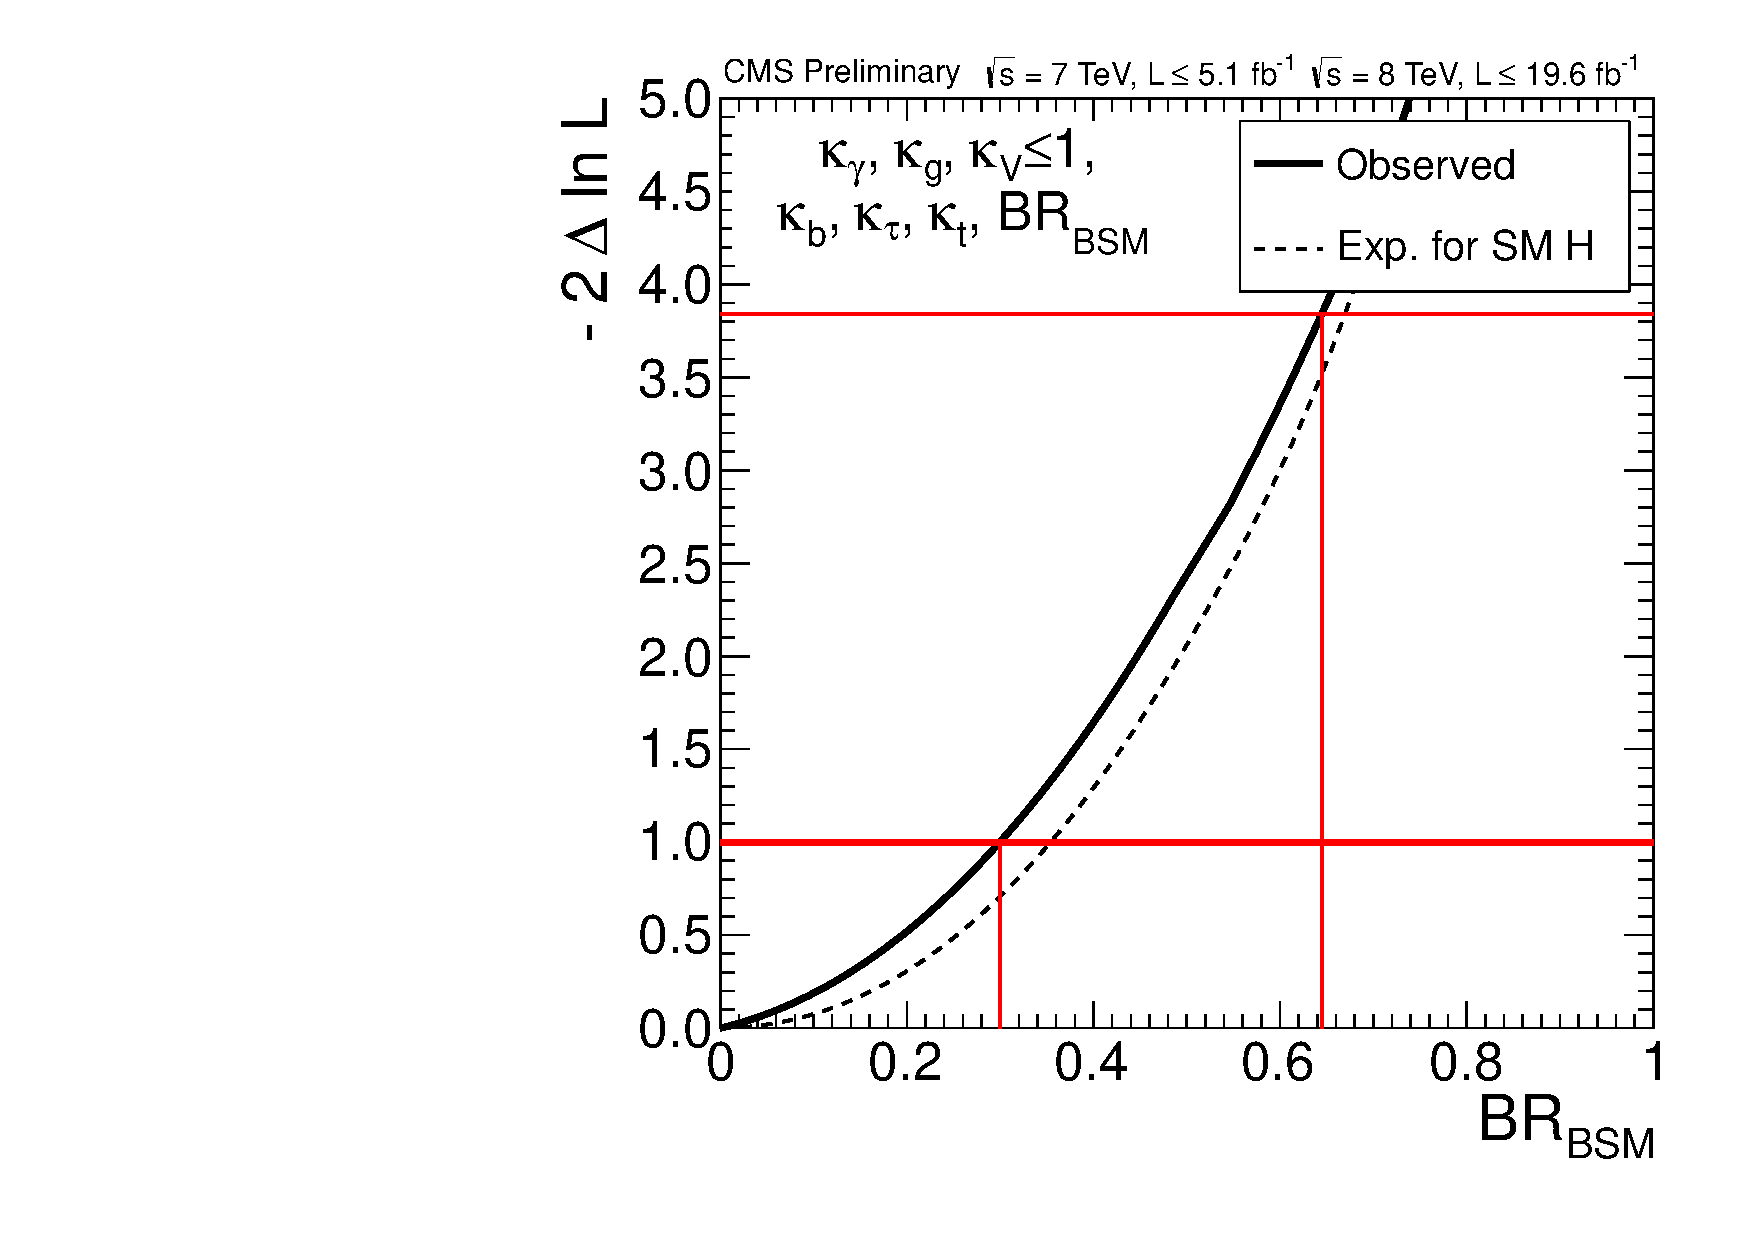
\includegraphics[width=\textwidth]{TalkPics/invbr.pdf}
  \end{columns}
\end{frame}

%OVERALL STRATEGY
\begin{frame}
  \frametitle{Measurement Strategy}
  \begin{columns}
    \column{.5\textwidth}
    \centering
    \begin{block}{\scriptsize Select VBF Topology}
      \scriptsize
      \begin{itemize}
      \item 2 jets with a large $\eta$ separation
      \item Nothing in the gap between the jets
      \item Need dedicated VBF trigger
      \end{itemize}
    \end{block}
    \vspace{0.5cm}
    \begin{figure}
    \begin{fmfgraph*}(100,70)
      \fmftop{i1,m1,o1}
      \fmfbottom{i2,o2}
      \fmf{fermion}{v1,o2}
      \fmf{fermion}{v1,i2}
      \fmf{dashes,label=$H$}{v1,m1}
      \fmflabel{$jet$}{i2}
      \fmflabel{$jet$}{o2}
      \fmflabel{$MET$}{m1}
    \end{fmfgraph*}
    \end{figure}

    \column{.5\textwidth}
    \scriptsize
    \begin{block}{}
      \begin{itemize}
      \item Clean data from pileup and mismeasured MET
      \item Use hard cuts to restrict backgrounds
      \item Remaining background estimation must be data driven as hard cuts make MC unreliable
      \item This iteration just a counting experiment, shape based analysis planned for final paper with parked data
      \end{itemize}
    \end{block}
  \end{columns}
\end{frame}

\begin{frame}
  \frametitle{Backgrounds Overview}
  \begin{columns}
    \column{.6\textwidth}
    \vspace{-0.3cm}
    \begin{block}{\scriptsize Main backgrounds:}
      \scriptsize
      \begin{itemize}
      \item $W$ + jets where lepton is missed
      \item[-] {\color{red}AM+Patrick cross check $W\rightarrow e/\mu$ \& measure $W\rightarrow\tau_{h}$ background from data}
      \item $Z\rightarrow\nu\nu$ + jets
      \item QCD: {\color{red}Sasha}
      \end{itemize}
    \end{block}
    \vspace{-0.3cm}
    \begin{block}{\scriptsize Data driven $W/Z$ + jets estimation:}
      \scriptsize
      \begin{itemize}
      \item Pick $W/Z$ dominated control region in same trigger sample with same VBF selection
      \item Recalculate MET after removing leptons from $W$ \& $Z$
      \item[-] Mimics $W$ with missed leptons/$Z\rightarrow\nu\nu$
      \item Check data/MC agreement in control regions
      \item Assume MC signal/control ratio is the same as that in data
      \end{itemize}
    \end{block}
    \column{.05\textwidth}
    \column{.35\textwidth}
    %WJETS
    \begin{fmfgraph*}(75,60)
      \fmftop{i1,m1,m2,o1}
      \fmfbottom{i2,o2}
      \fmf{fermion,label=$e/\mu/\tau$,label.side=left}{v2,m1}
      \fmf{fermion,label=$\nu$,label.side=right}{v2,m2}
      \fmf{photon,tension=7/5,label=$W$}{v1,v2}
      \fmf{fermion}{v1,i2}
      \fmf{fermion}{v1,o2}
      \fmflabel{$jet$}{i2}
      \fmflabel{$jet$}{o2}
    \end{fmfgraph*}
    \vspace{0.2cm}
    %ZJETS
    \begin{fmfgraph*}(75,50)
      \fmftop{i1,m1,m2,o1}
      \fmfbottom{i2,o2}
      \fmf{fermion}{v1,i2}
      \fmf{fermion}{v1,o2}
      \fmf{photon,tension=7/5,label=$Z$}{v1,v2}
      \fmf{fermion,label=$\nu$,label.side=left}{v2,m1}
      \fmf{fermion,label=$\nu$,label.side=right}{v2,m2}
      \fmflabel{$jet$}{i2}
      \fmflabel{$jet$}{o2}
    \end{fmfgraph*}
    
    %QCD
    \begin{fmfgraph*}(75,60)
      \fmftop{i1,m1,m2,m3,m4,o1}
      \fmfbottom{i2,o2}
      \fmf{fermion,tension=4}{v1,i2}
      \fmf{fermion,tension=4}{v1,o2}
      \fmf{fermion,label=$jets$,label.side=left}{v1,m1}
      \fmf{fermion}{v1,m2}
      \fmf{fermion}{v1,m3}
      \fmf{fermion}{v1,m4}
      \fmflabel{$jet$}{i2}
      \fmflabel{$jet$}{o2}
    \end{fmfgraph*}
  \end{columns}
\end{frame}

%TRIGGER AND DATASETS
\begin{frame}
  \frametitle{Datasets and Trigger}
  \begin{columns}
    \column{.5\textwidth}
    \vspace{-0.2cm}
    \begin{block}{\scriptsize Datasets:}
      \scriptsize
      \begin{itemize}
      \item 8 TeV MET datasets
      \item[-] Total of 19.6 $fb^{-1}$
      \item MET filters are used to cut out events with mismeasured MET
      \end{itemize}
    \end{block}
    \vspace{-0.3cm}
    \begin{block}{\scriptsize Trigger:}
      \scriptsize
      \begin{itemize}  
      \item HLT\_DiPFJet40\_PFMET noMu65\_MJJ800VBF\_AllJets
      \item[-] VBF means $|\Delta \eta_{j_{1}j_{2}}| > 3.5 $
      \item {\color{red} IC heavily involved in design of the trigger}
      \end{itemize}
    \end{block}
    \column{.5\textwidth}
    \centering
    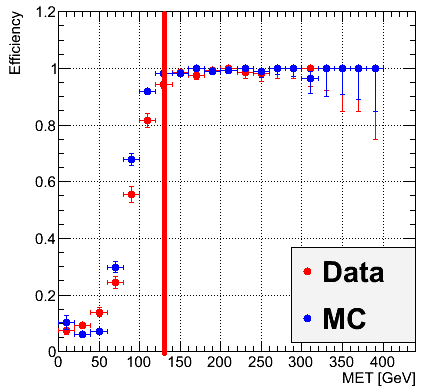
\includegraphics[height=.45\textheight]{TalkPics/METtrig.png}
    
    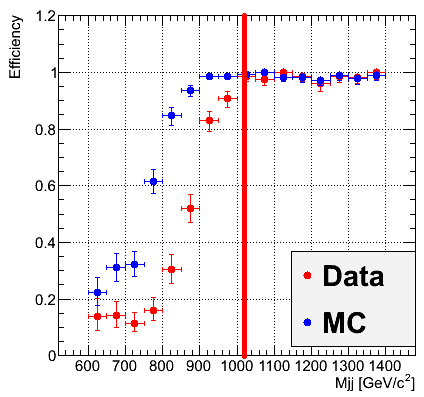
\includegraphics[height=.45\textheight]{TalkPics/Mjjtrig.png}
  \end{columns}
\end{frame}

%OBJECTS
\begin{frame}
  \frametitle{Objects}
  \begin{columns}
    \column{.5\textwidth}
    \begin{block}{\scriptsize VBF Selections}
      \scriptsize
      \begin{itemize}
      \item \color{red} Applied to all regions
      \item 2 jets:
      \item[-] Both jets must pass loose PUJetID
      \item[-] $p_{T} > 50 GeV$,  $|\eta| < 4.7$
      \item[-] $|\Delta\eta|>4.2$ , $\eta_{j_{1}}*\eta_{j{_2}}<0$
      \item[-] $m_{jj} > 1200 GeV$
      \end{itemize}
    \end{block}
    \begin{block}{\scriptsize MET}
      \scriptsize
      \begin{itemize}
      \item Using Type 0 + 1 Corrections
      \end{itemize}
    \end{block}
    \column{.5\textwidth}
    \begin{block}{\scriptsize Electrons}
      \scriptsize
      \begin{itemize}
        \item Veto:
        \item[-] $p_{T}>10 GeV$, $|\eta<2.5|$
        \item[-] rel PF Iso $< 0.2$
        \item Tight:
        \item[-] $p_{T}>20 GeV$, $|\eta<2.5|$
      \end{itemize}
    \end{block}
    \begin{block}{\scriptsize Muons}
      \scriptsize
      \begin{itemize}
        \item Veto:
        \item[-] $p_{T}>10 GeV$, $|\eta<2.1|$
        \item[-] rel PF Iso $< 0.2$
        \item Tight: 
        \item[-] $p_{T}>20 GeV$, $|\eta<2.1|$
      \end{itemize}
    \end{block}
  \end{columns}
\end{frame}

%SIGNAL EVENT SELECTION
\begin{frame}
    \frametitle{Signal Event Selection}
  \vspace{-0.2cm}
  \begin{block}{\scriptsize Signal Region Selection:}
    \scriptsize
    \begin{itemize}
    \item PFMET $> 130GeV$ \& $\Delta\phi_{jj}<1.0$ to reduce QCD
    \item $e/\mu$ veto to reduce $W/Z$+jets
      \end{itemize}
  \end{block}
  \vspace{-0.15cm}
  \scriptsize Data MC difference is QCD
  \begin{columns}
    \column{.5\textwidth}
    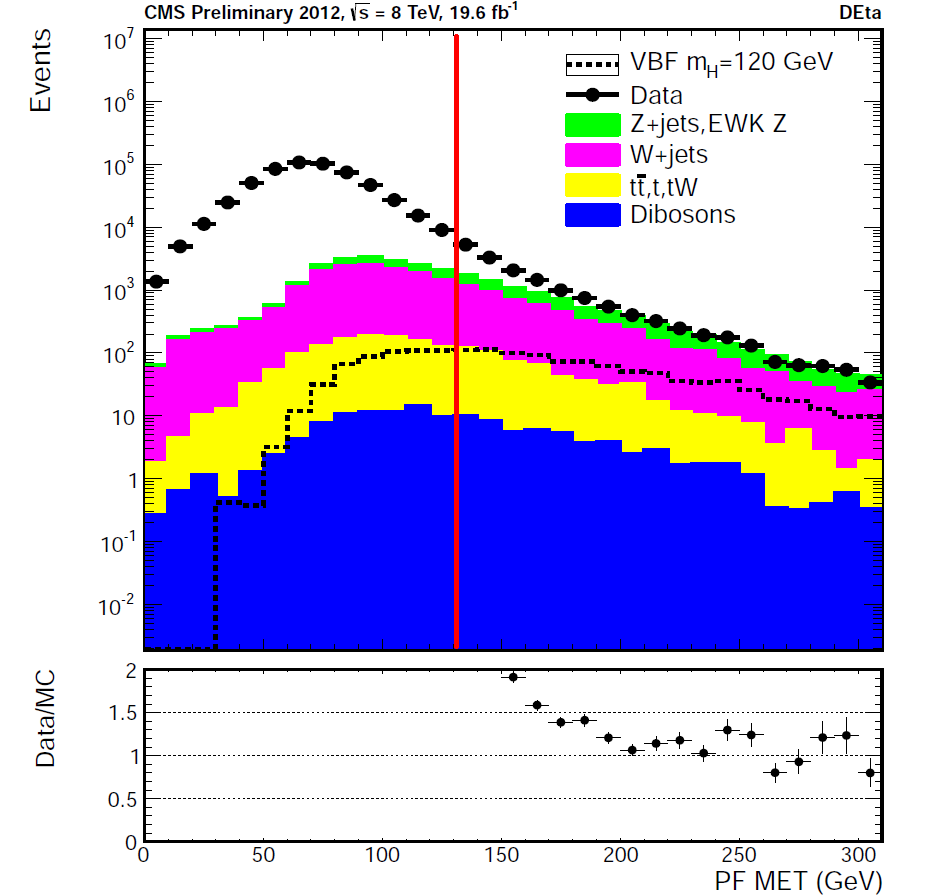
\includegraphics[width=\textwidth,height=.5\textheight]{TalkPics/met_DEta_nunu.png}
    \column{.5\textwidth}
    
    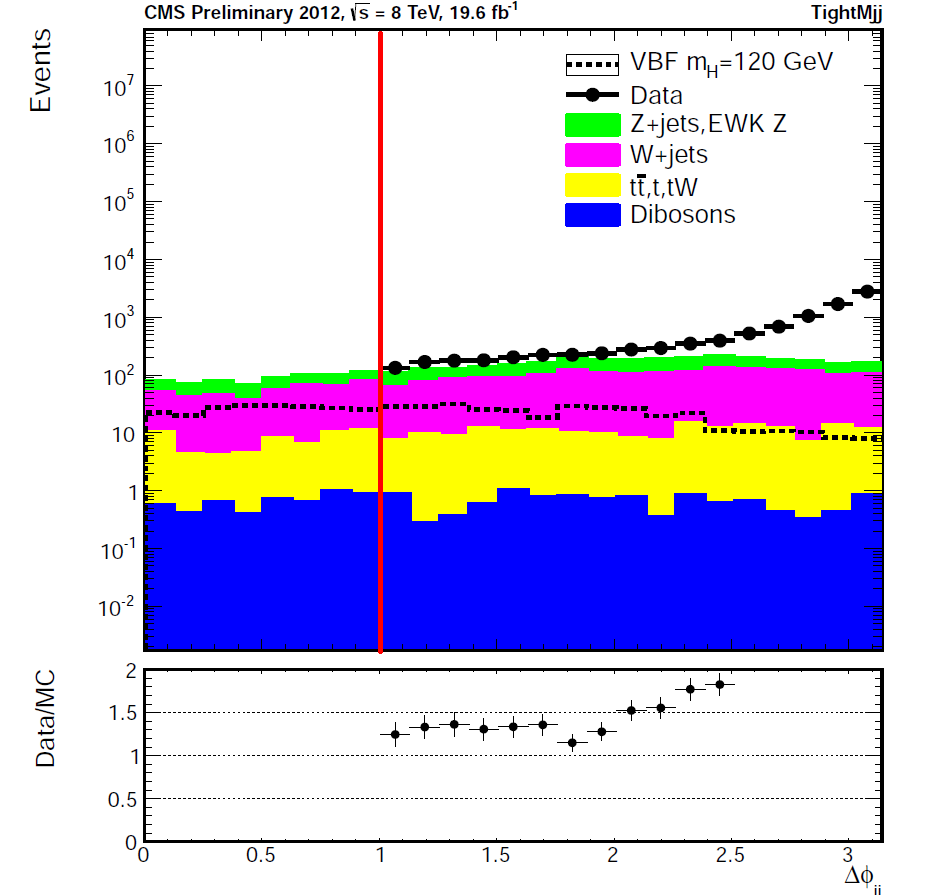
\includegraphics[width=\textwidth,height=.5\textheight]{TalkPics/dphijj_TightMjj_nunu.png}
  \end{columns}
\tiny
\vspace{-0.1cm}
\begin{block}{}
\centering
\begin{tabular}{|l|p{0.07\textwidth}|p{0.07\textwidth}|p{0.07\textwidth}|p{0.07\textwidth}||p{0.07\textwidth}|c||p{0.07\textwidth}|}

\hline

Top & W+jets & Z+jets & VV & SumMC & Data & Signal 120 \\

\hline

$  55 \pm 6 $ & $ 382 \pm 18 $ & $ 258 \pm 10 $ & $ 5.2 \pm 0.6 $ & $ 700.2 \pm 21.5 $ & XXX & $ 209 \pm 9 $ \\

\hline

\end{tabular}
\end{block}
\end{frame}

%BACKGROUNDS

%Background estimations!
\begin{frame}
  \frametitle{$W$+jets Background Estimation}
  \vspace{-0.4cm}
  \begin{columns}
    \column{.5\textwidth}
    \begin{block}{\scriptsize Background estimation formula:}
      \scriptsize
      \centering
      $N^{S}_{data} (W\rightarrow e/\mu) = (N^{C}_{data}-N^{C}_{bkg})\frac{N^{S}_{MC}}{N^{C}_{MC}}$  
    \end{block}
    \column{.5\textwidth}
    \begin{block}{\scriptsize $W \rightarrow \mu/ e$ Control Region Selection:}
      \scriptsize
      \begin{itemize}
      \item 1 tight muon/electron:
      \item MET without $(\mu/e)>130 GeV$
      \end{itemize}
    \end{block}
  \end{columns}
  \begin{columns}
    \column{.5\textwidth}
    \centering
    \scriptsize
    $W\rightarrow e\nu$

    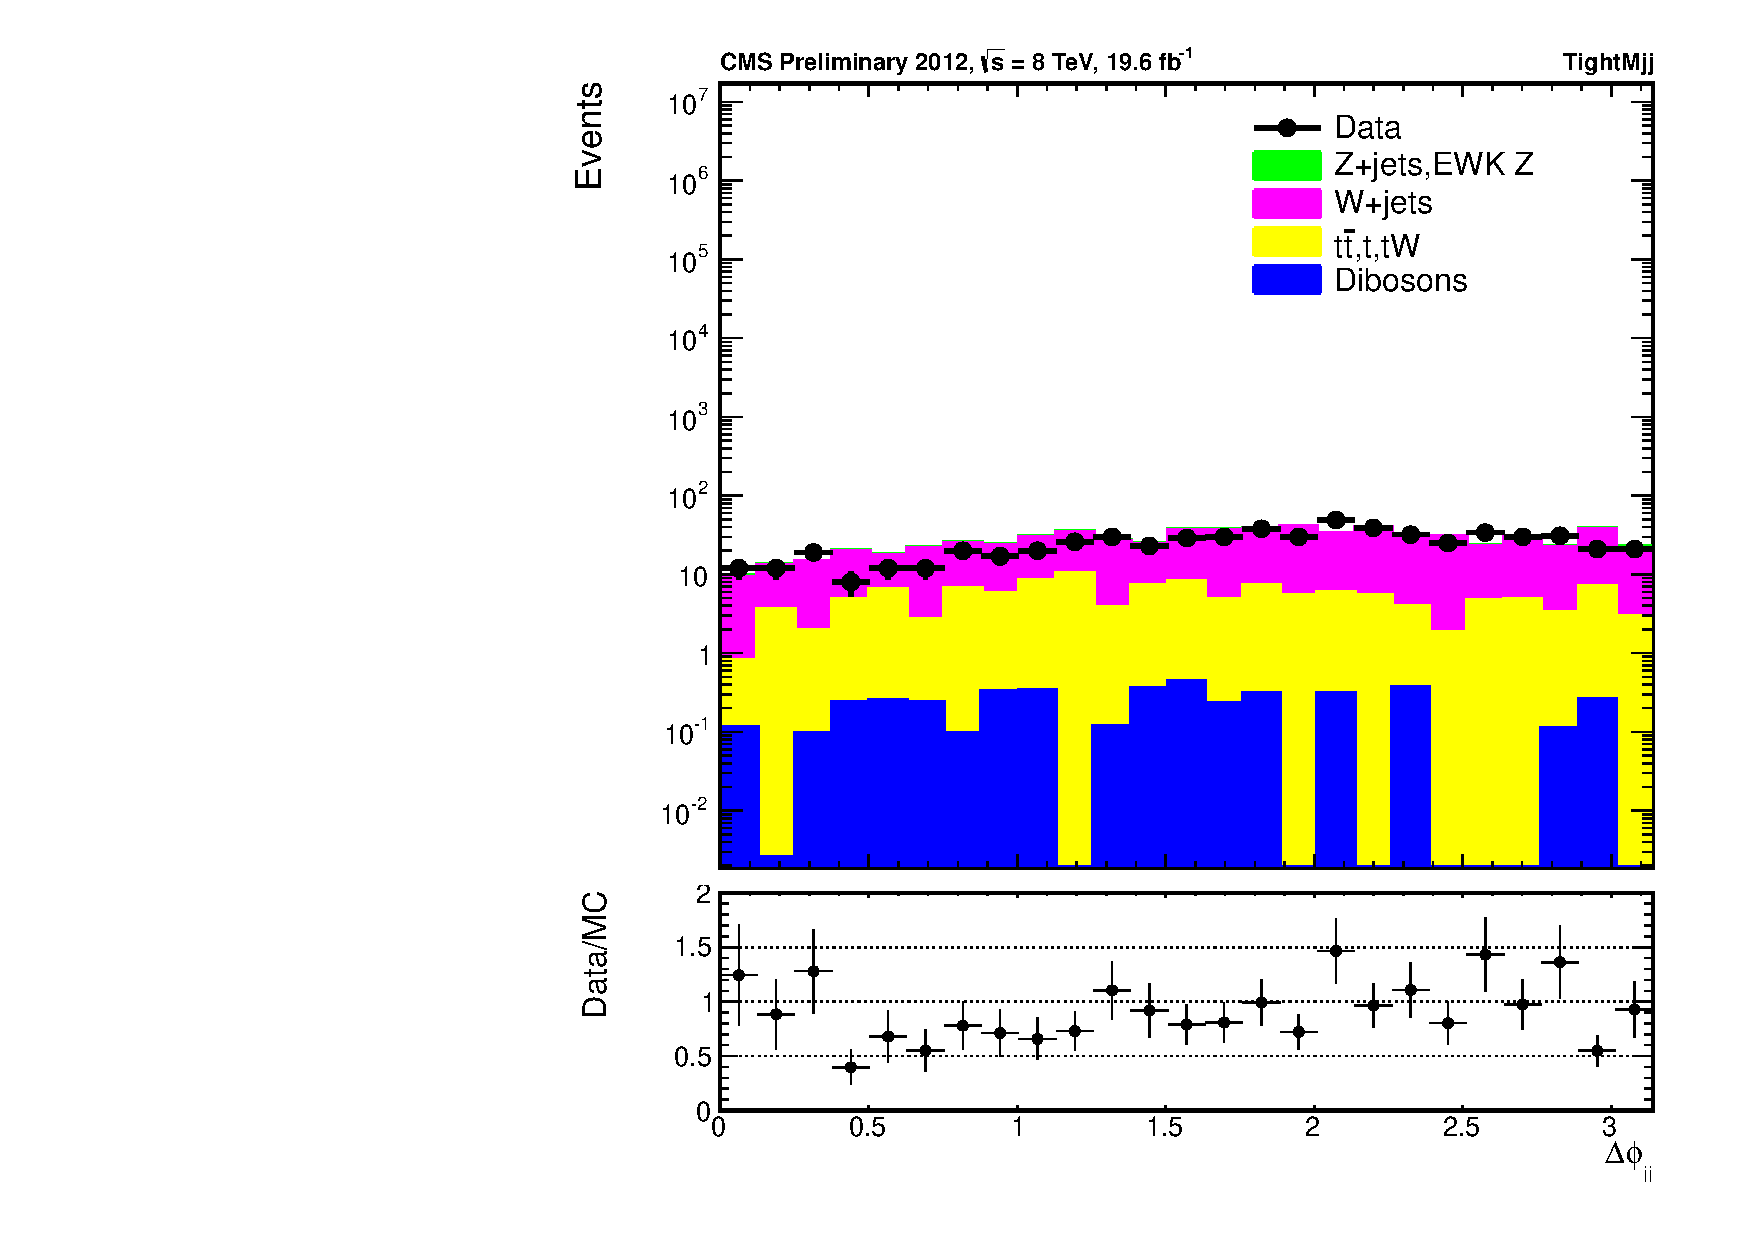
\includegraphics[width=\textwidth,height=.5\textheight]{TalkPics/dphijj_TightMjj_enu.pdf}
    \column{.5\textwidth}
    \centering
    \scriptsize
    $W\rightarrow \mu\nu$

    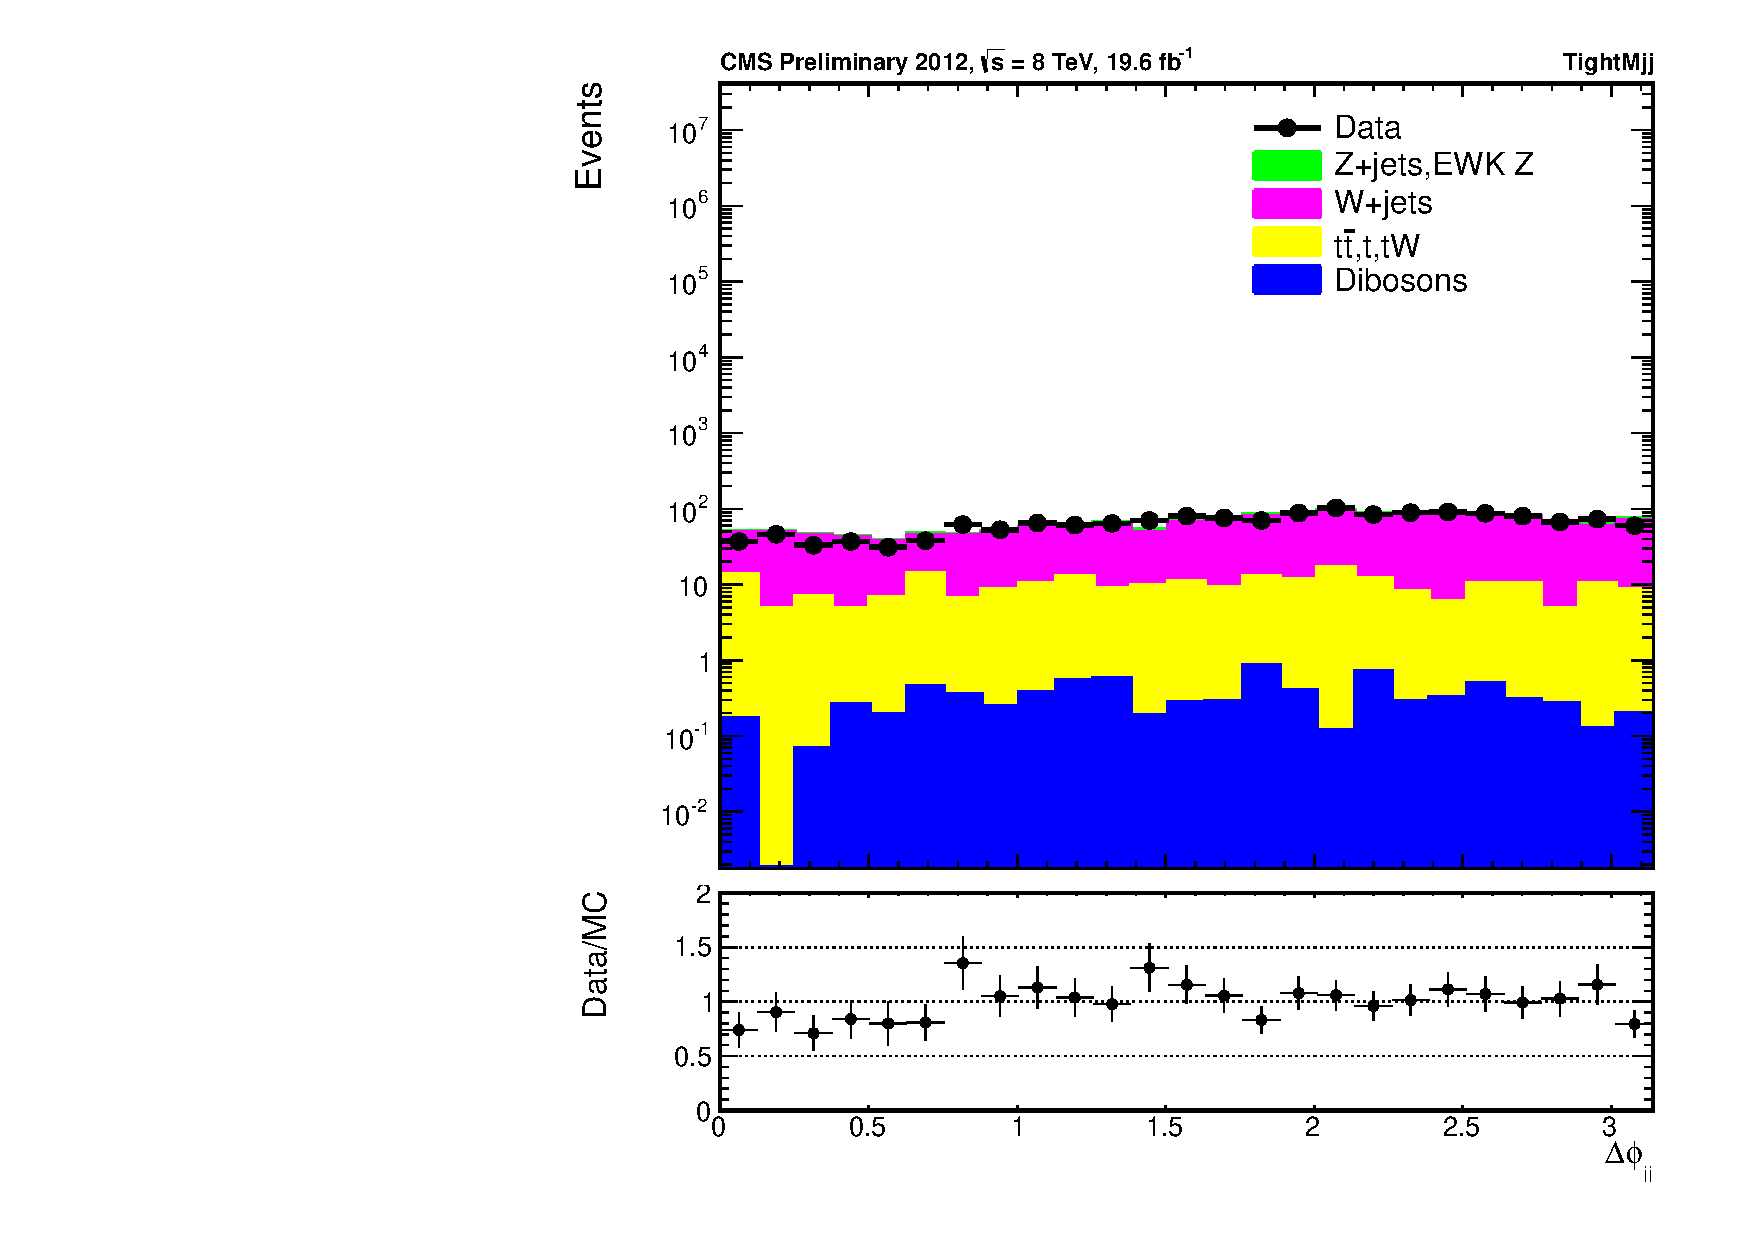
\includegraphics[width=\textwidth,height=.5\textheight]{TalkPics/dphijj_TightMjj_munu.pdf}
  \end{columns}
  \vspace{-0.2cm}
  
  \begin{columns}
    \column{.5\textwidth}
    \begin{block}{}
      \scriptsize
      \centering
      $N^{S}_{MC}=$ $142\pm11(stat.)$ events

      $N^{S}_{data} =$ $87\pm17(stat.)$ events
    \end{block}
    \column{.5\textwidth}
    \begin{block}{}
      \scriptsize
      \centering
      $N^{S}_{MC} =$ $130\pm10$ events

      $N^{S}_{data} =$ $105\pm13(stat.)$ events
    \end{block}
  \end{columns}
\end{frame}

\begin{frame}
  \frametitle{$W\rightarrow\tau$ Background Estimation}
  \begin{columns}
    \column{.5\textwidth}
    \vspace{-0.3cm}
    \vspace{-0.2cm}
    \begin{block}{\scriptsize $W\rightarrow \tau$ Method:}
      \scriptsize
      \begin{itemize}
      \item Select subsample of signal region
      \item Require 1 $\tau_{hadronic}$ candidate
      \item[-] $p_T>20 GeV$, $|\eta|<2.3$
      \item[-] Discriminant ``byTightCombinedIsolationDeltaBetaCorr3Hits''
      \item Correct with the efficiency: 0.55
      \item Fake rate: 0.02/0.03 in barrel/endcap
      \end{itemize}
    \end{block}
    \vspace{-0.2cm}
    \begin{block}{\scriptsize Result}
      \scriptsize
      \begin{itemize}
      \item MC expectation: $130\pm10$
      \item $N^{data}_{W\rightarrow\tau\nu} = 135 \pm 52(stat)\pm11(syst)$
      \end{itemize}
    \end{block}
    \column{.5\textwidth}
    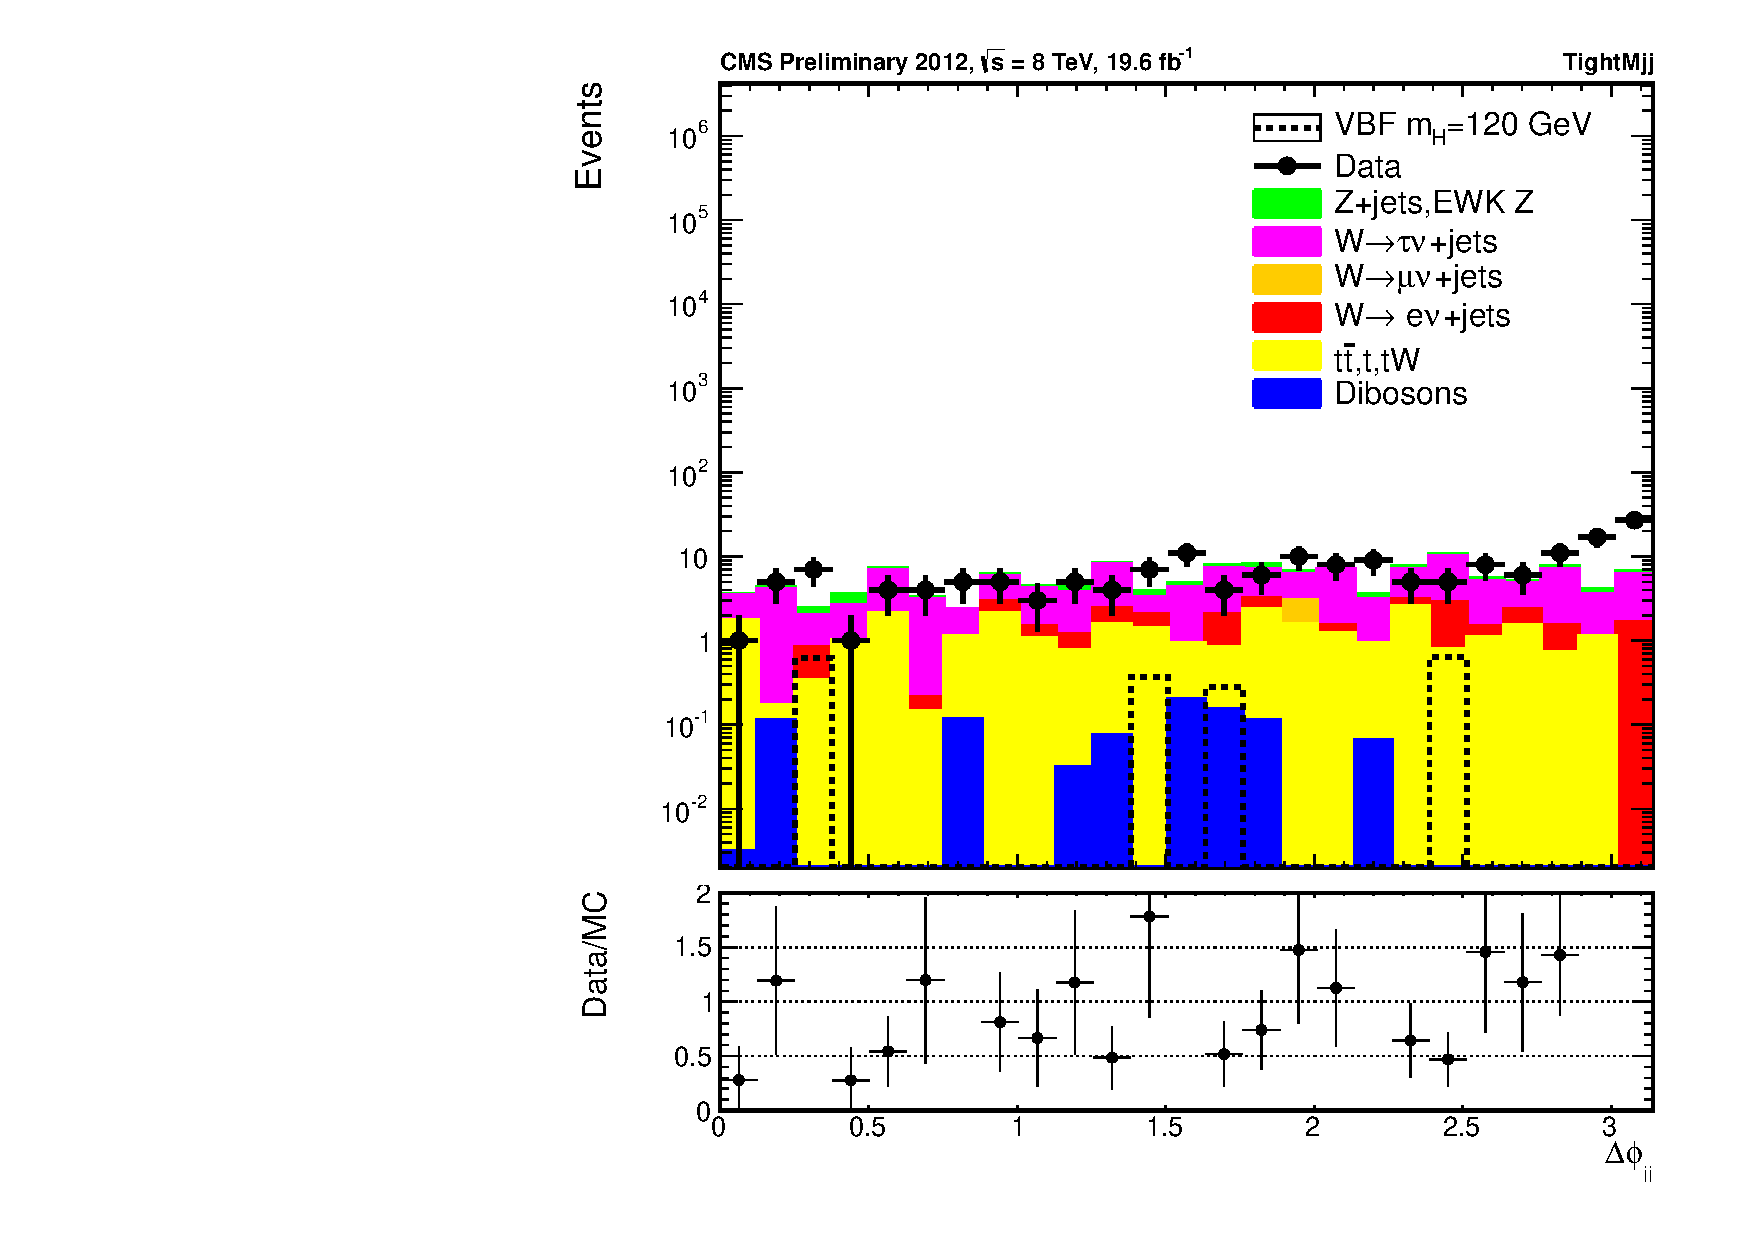
\includegraphics[width=\textwidth]{TalkPics/wtaudphiplot.pdf}

    \scriptsize
    Thanks to A. Gilbert and M. Acosta for explanations of tau id
  \end{columns}
\end{frame}

\begin{frame}
  \frametitle{Systematics}
  {\color{red} IC doing $W$ + jets uncertainties:} work in progress
  \begin{columns}
  %%   \column{.5\textwidth}
  %%   \centering
  %%   \hspace{-0.4cm}
  %%   \begin{block}{\scriptsize Background Uncertainties:}
  %%     \tiny
  %%     \begin{tabular}{|l|c|}
  %%       \hline
  %%       Source & Uncertainty \\
  %%       \hline
  %%       Statistics in $Z$ region & 25\% \\
  %%       Statistics in $W\rightarrow e$ region & 10\% \\
  %%       Statistics in $W\rightarrow \mu$ region & 5\% \\
  %%       $W$ MC statistics & 10\% \\
  %%       Luminosity & \\ 4\%
  %%       Jet energy scale & 3\% \\
  %%       Jet energy resolution & not included yet \\
  %%       Unclustered energy scale & not included yet \\
  %%       \hline
  %%     \end{tabular}
  %%   \end{block}
  %%   \begin{block}{\scriptsize Signal Uncertainties}
  %%     \tiny
  %%     \begin{tabular}{|l|c|}
  %%       \hline
  %%       Source & Uncertainty \\
  %%       \hline
  %%       Jet energy scale & 10\% \\
  %%       Jet energy resolution & not included yet \\
  %%       Unclustered energy scale & not included yet \\
  %%       \hline
  %%     \end{tabular}      
  %%   \end{block}
    \column{.3\textwidth}
    \begin{block}{\scriptsize Uncertainties considered}
      \scriptsize
      \begin{itemize}
      \item Statistics
      \item Jet Energy Scale(JES)
      \item Jet Energy Resolution(JER)
      \item Unclustered Energy Scale
      \item Pileup ID
      \item Luminosity
      \end{itemize}
    \end{block}
    \column{.7\textwidth}
    \hspace{-0.4cm}
    \begin{block}{\scriptsize Preliminary $W$ + Jets Background Uncertainties}
      \scriptsize
      \centering
      \begin{tabular}{|l|| c| c| }
        \hline
        $N_{W\rightarrow e\nu}^{data}$ & Electron & Muon \\
        \hline
        Central num. of events & 87 & 105  \\
        Statistical & $\pm$19.8\% & $\pm$12.2\% \\
        JESUP & -3.75\% & +4.6\% \\
        JESDOWN & +3.57\% & +1.91\% \% \\
        JERBETTER & +2.91\% & -0.616\%  \\
        JERWORSE & +7.01\% & +6.84\%  \\
        \hline
      \end{tabular}
    \end{block}
  \end{columns}
\end{frame}



\begin{frame}
  \frametitle{$Z$+jets Background Estimation}
  \begin{block}{\scriptsize Z+jets background estimation formula:}
    \scriptsize 
    \centering
    $N^{S}_{data}(Z\rightarrow\nu\nu)=(N^{C}_{data} - N^{C}_{bkg})\frac{\sigma(Z\rightarrow\nu\nu)}{\sigma(Z/\gamma^{*}\rightarrow\mu\mu)}\frac{\epsilon^{S}_{VBF}/\epsilon^{C}_{VBF}}{\epsilon_{\mu\mu}}$
  \end{block}
  \begin{columns}
    \column{.5\textwidth}
    \begin{block}{\scriptsize $Z\rightarrow\nu\nu$ Control Region Selection:}
      \tiny
      \begin{itemize}
      \item Select $Z\rightarrow\mu\mu$ and extrapolate to $Z\rightarrow\nu\nu$
      \item 2 tight muons
      \item MET after $Z$ candidate removed $> 130 GeV$
      \item No additional veto muons/electrons
      \end{itemize}
    \end{block}
    \begin{block}{}
      \centering
      \scriptsize
      $N^{S}_{data}=162\pm48$
    \end{block}
    \column{.5\textwidth}
    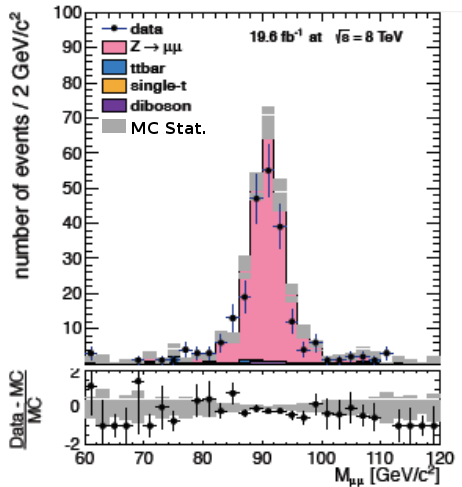
\includegraphics[width=.8\textwidth]{TalkPics/zcontrol.png}
  \end{columns}
\end{frame}

%QCD
\begin{frame}
  \frametitle{QCD}
  \begin{columns}
    \column{.5\textwidth}
    \begin{block}{\scriptsize QCD Background Strategy}
      \scriptsize
      \begin{itemize}
      \item Critical part of analysis
      \item V. low MC statistics
      \item Therefore two options:
      \item[1)] Estimate from data
      \item[2)] Reduce background further
      \end{itemize}
    \end{block}
    \begin{block}{\scriptsize QCD Control Region Selection}
      \scriptsize
      \begin{itemize}
      \item $\Delta\phi_{jj}>2.6$  
      \end{itemize}
    \end{block}
    \column{.5\textwidth}
    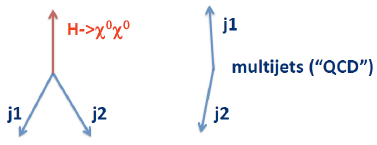
\includegraphics[width=\textwidth]{TalkPics/qcddiag.png}
    
    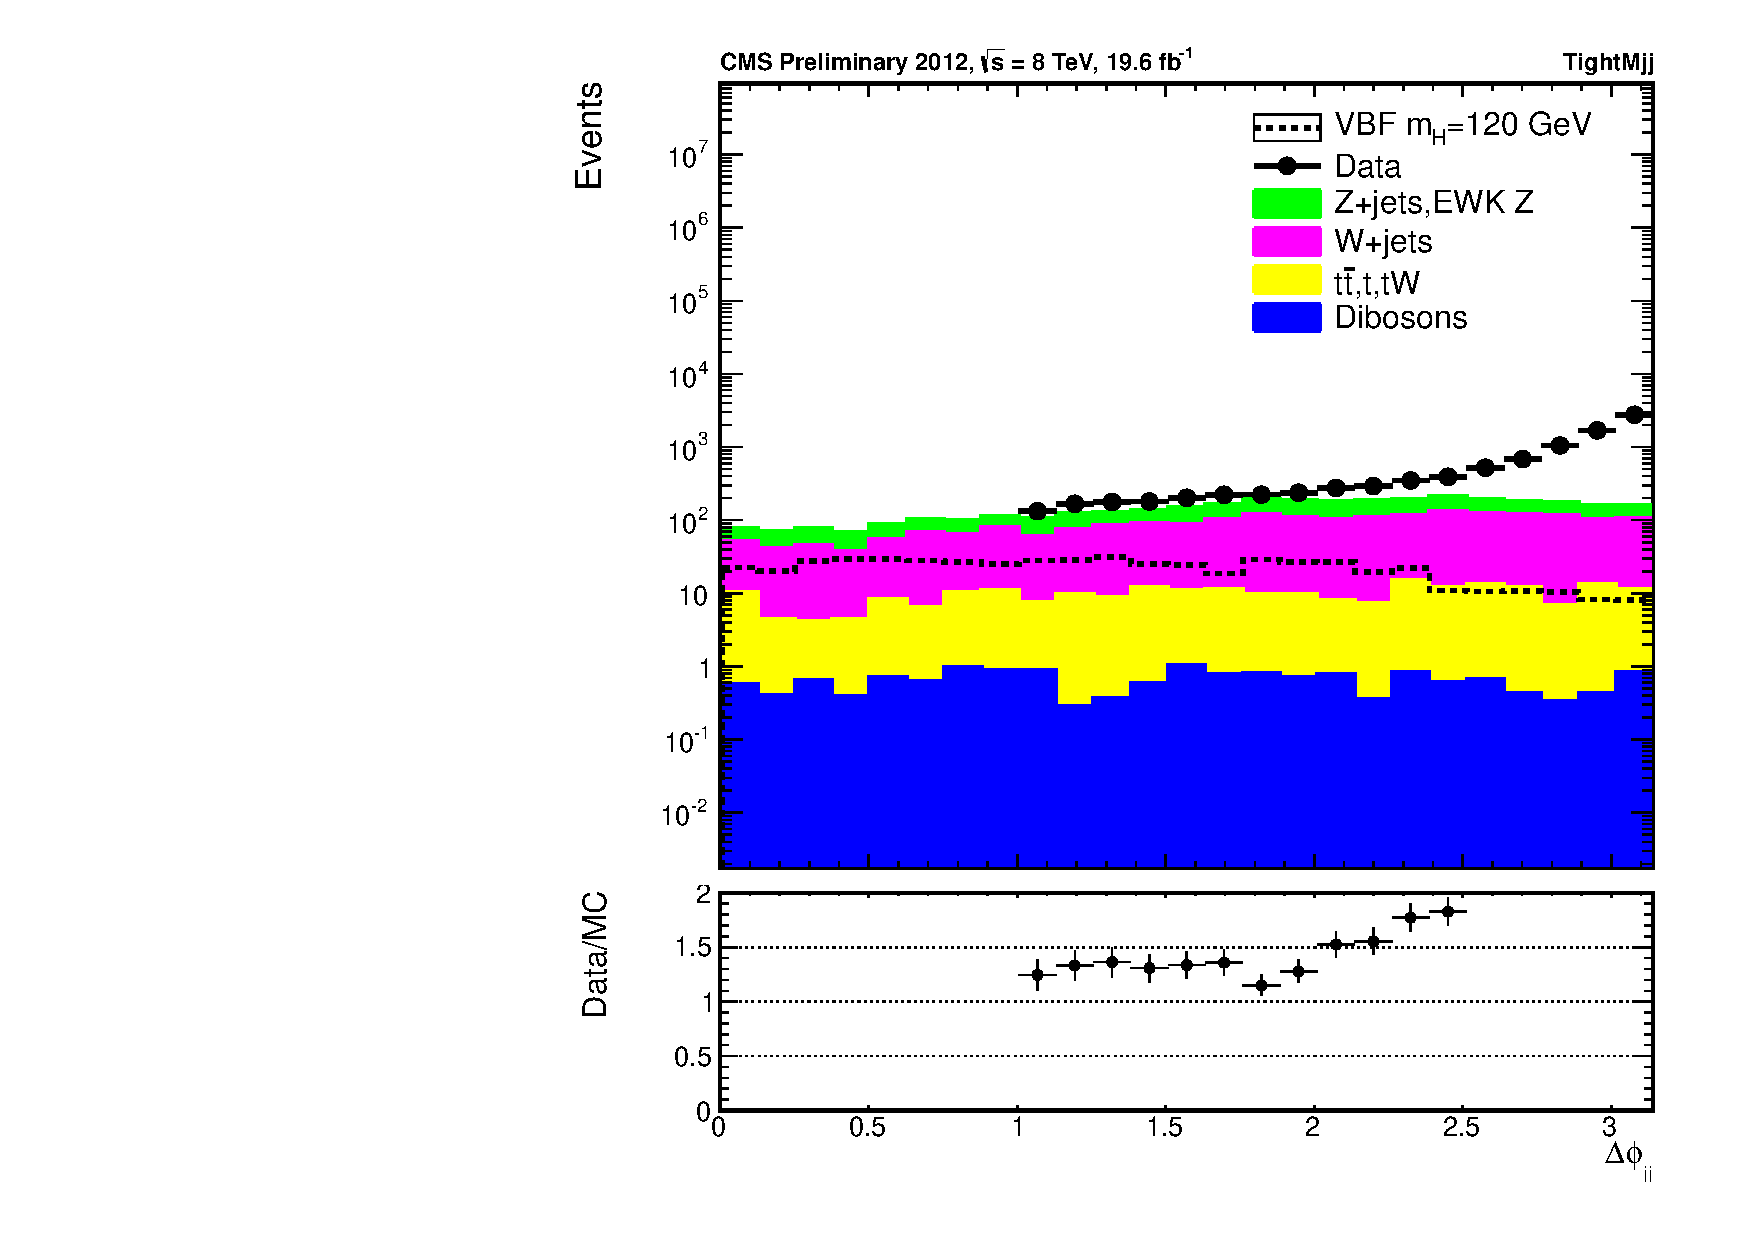
\includegraphics[width=\textwidth,height=.6\textheight]{TalkPics/dphijj_TightMjj_nunu.pdf}
  \end{columns}
\end{frame}

\begin{frame}
  \frametitle{QCD Background Estimation - Method 1}
  \begin{columns}
    \column{.5\textwidth}
    \begin{block}{\scriptsize Formula:}
      \scriptsize
      \centering
      $N^{S}_{multijet} = (N^{C}-N_{non-multijet})xr$
      \vspace{0.3cm}

      $r=\frac{N_{data}(\Delta\phi_{jj}<1.0) - N_{non-multijet}(\Delta\phi_{jj}<1.0)}{N_{data}(\Delta\phi_{jj}>2.6)-N_{non-multijet}(\Delta\phi_{jj}>2.6)}$
    \end{block}
    
    \begin{block}{\scriptsize Method:}
      \scriptsize
      \begin{itemize}
      \item Extrapolate from $\Delta\phi_{jj}>2.6$ to $\Delta\phi_{jj}<1.0$
      \item Preliminary study showed r appeared flat
      \item After more analysis method is not usable
      \end{itemize}
    \end{block}
      
    \column{.5\textwidth}
    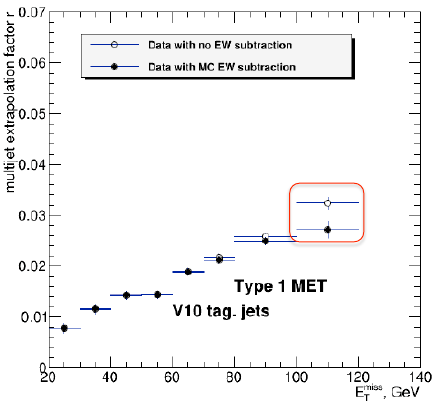
\includegraphics[width=\textwidth]{TalkPics/qcdplot.png}
  \end{columns}
\end{frame}

\begin{frame}
  \frametitle{QCD Background Estimation - Method 2}
  \begin{columns}
    \column{.5\textwidth}
    \begin{block}{\scriptsize Method:}
      \scriptsize
      \begin{itemize}
      \item Find a distribution that is the same shape in $\Delta\phi_{jj}<1.0$ and $\Delta\phi_{jj}>2.6$ regions
      \item[-] We use MET
      \item Normalise below MET cut and extrapolate
      \item If you shift control region distribution by 10 GeV they look similar but still not entirely satisfactory
      \end{itemize}
    \end{block}
    \column{.5\textwidth}
    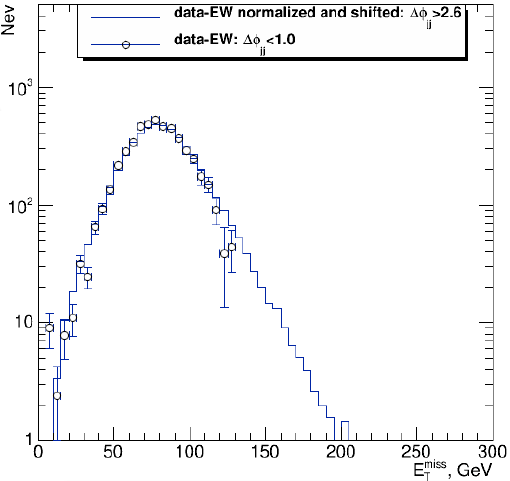
\includegraphics[width=\textwidth,height=.45\textheight]{TalkPics/qcdplot2.png}
    
    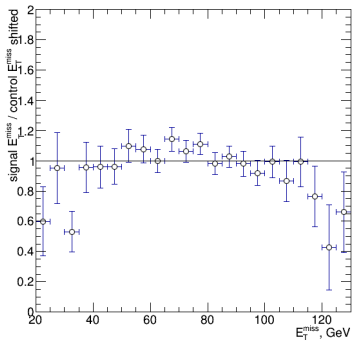
\includegraphics[width=\textwidth,height=.45\textheight]{TalkPics/qcdplot2ratio.png}
  \end{columns}
\end{frame}

\begin{frame}
  \frametitle{Reducing QCD Contribution}
  \begin{block}{\scriptsize Other Solutions}
      \scriptsize
      \begin{itemize}
      \item Given estimation has issues try cutting most of QCD so large estimation errors are less important
      \item Work in progress!
      \item Several options:
      \item Central Jet Veto (CJV)
      \item[-] Veto events with additional jets above a $p_{T}$ threshold between VBF Jets
      \item Additional Jet Veto
      \item[-] Veto additional jets above a $p_{T}$ threshold in the tracker region
      \item Variables used for SUSY hadronic searches, e.g. $\alpha_{T}$
       
      \end{itemize}
    \end{block}

\end{frame}

%LIMIT PLOTS
\begin{frame}
  \frametitle{Preliminary Expected Limits - QCD Method 1}
  \centering
  \scriptsize
  \vspace{-0.2cm}
  \begin{columns}
    \column{.5\textwidth}
    \centering
    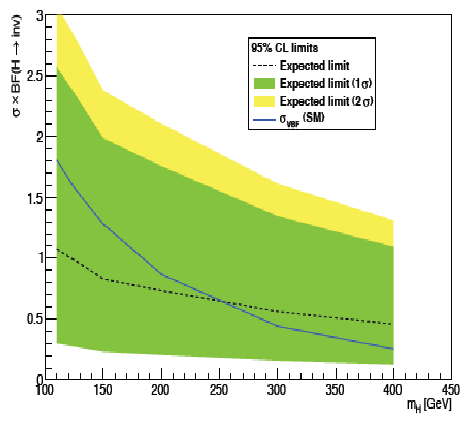
\includegraphics[width=\textwidth]{TalkPics/limitplot1.png}
    \column{.5\textwidth}
    \centering
    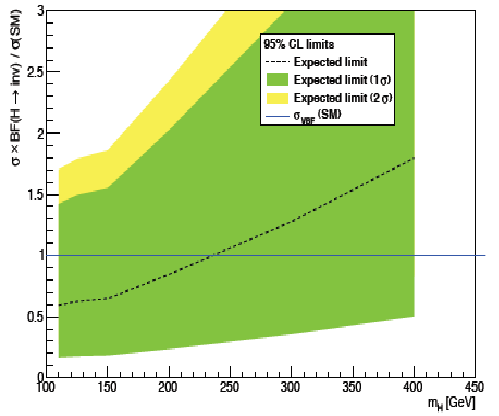
\includegraphics[width=\textwidth]{TalkPics/limitplot2.png}
  \end{columns}
  \vspace{-0.2cm}
  \begin{block}{}
    \scriptsize
    \begin{itemize}
    \item Very preliminary to make sure we can go to the end of the analysis
    \item Produced with combine package using $CL_{S}$ statistics, cross-checked with RooStats
    \item 95\% CL expected limit on the invisible BR for 125 GeV: 62\%
    \end{itemize}
  \end{block}
\end{frame}

\begin{frame}\label{lastframe}
  \frametitle{Summary}
  \begin{block}{}
  \begin{itemize}
  \item Most of the analysis is complete
  \item QCD still needs to be understood
  \item Some systematics still need to be included
  \item Expected limit on BR 62\% is promising and competitive with:
  \item[-] CMS ZH expected 79\% {\tiny (AN-13-116,AN-12-123)}
  \item[-] ATLAS ZH 65\% observed 84\% expected {\tiny (ATLAS-CONF-2013-011)}
  \item[-] CMS indirect observed 64\%
  \item Plan to have PAS for 8 TeV data then paper with additional parked data
  %OPTIMISATION AND CROSS-CHECKS
  \end{itemize}
  \end{block}
\end{frame}

\begin{frame}
  \frametitle{BACKUP}
\end{frame}

\begin{frame}
  \frametitle{Parked Data}
  \begin{itemize} 
  \item{\color{red} IC pushed strongly for data parking}    
  \item Jet $E_{T}>35(30) GeV$, $\Delta\eta_{jj}>3.5$, $m_{jj}>700 GeV$
  \item[-] Trigger with $E_{T}>30 GeV$ added for runs C+D
  \item Good efficiency for visible and invisible VBF Higgs channels
  \item Plan to update result with parked data included after PAS
  \end{itemize}
\end{frame}

\begin{frame}
  \frametitle{$W$+jets background $m_{T}$ plots}
  \begin{columns}
    \column{.33\textwidth}
    $e\nu$
    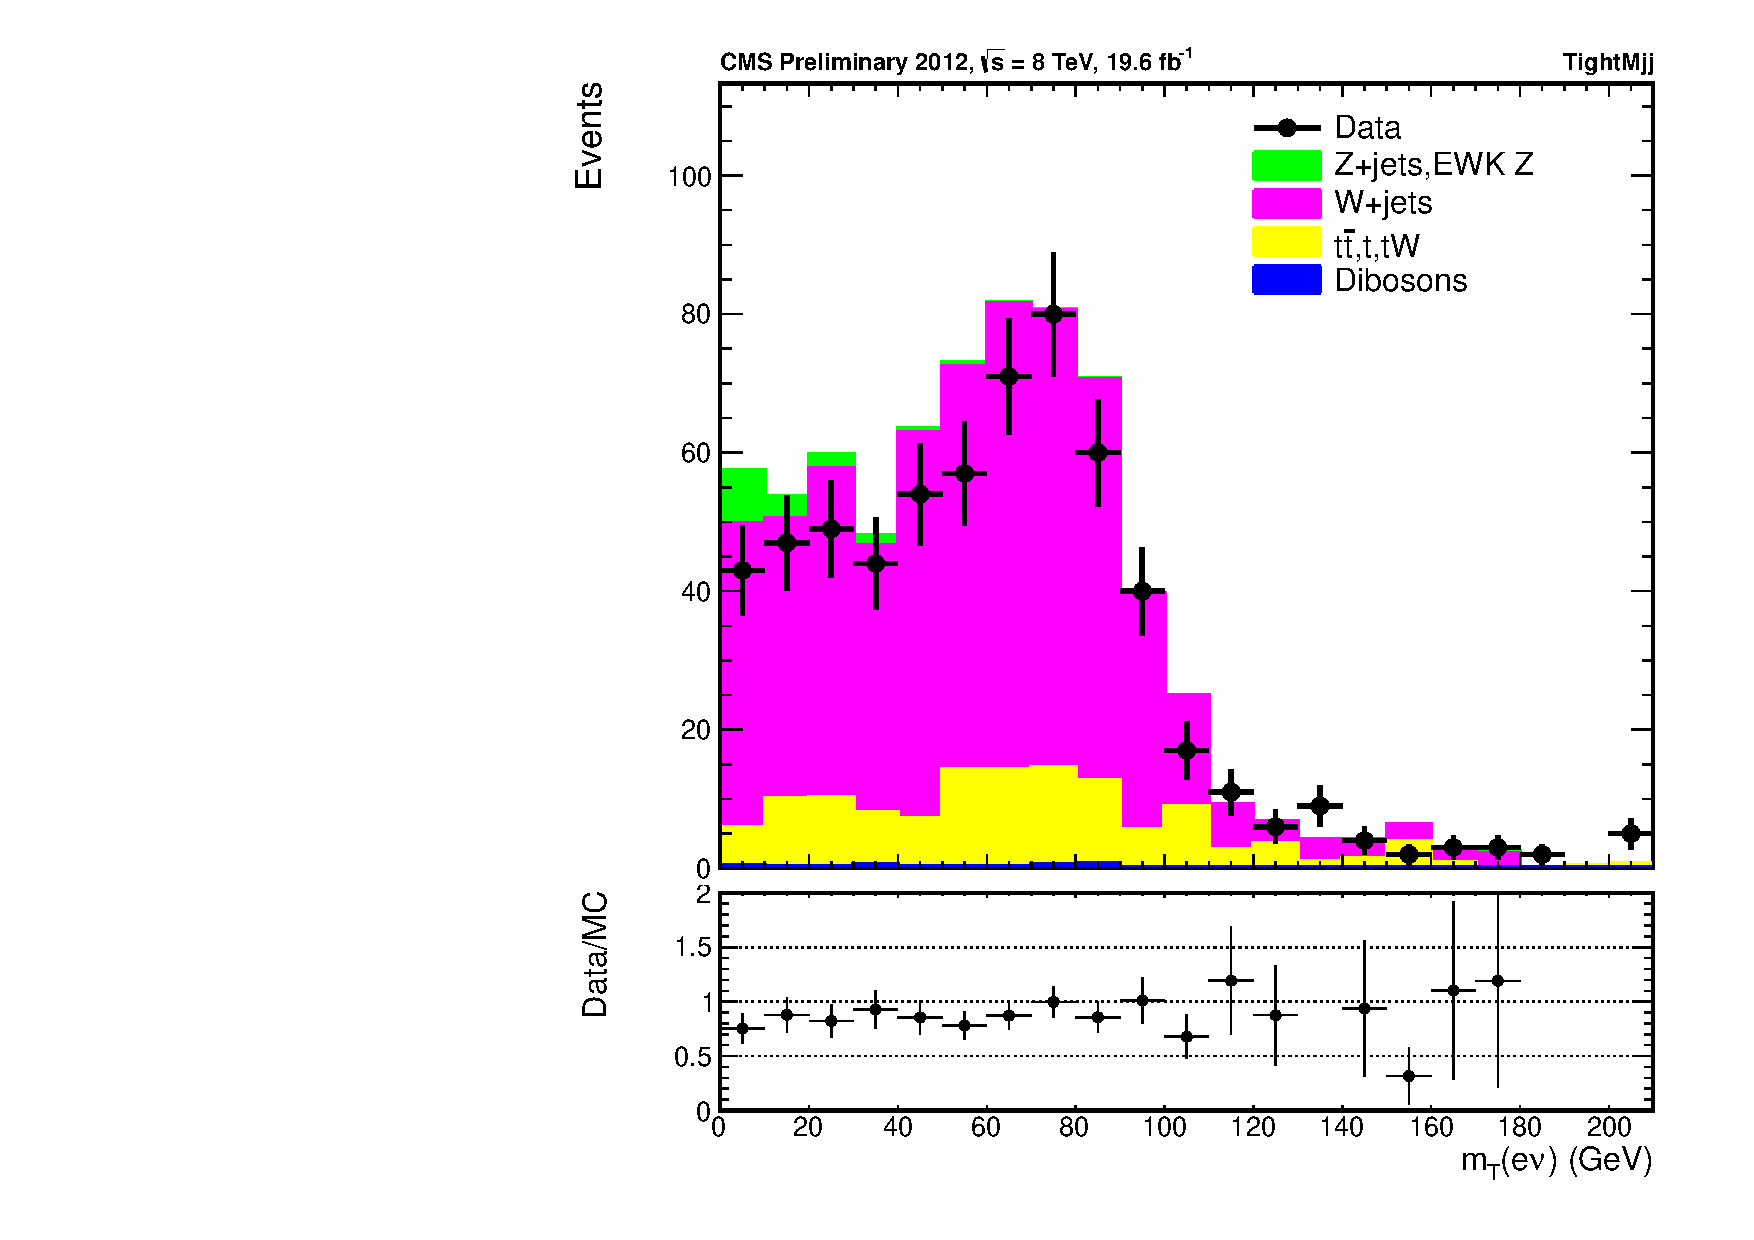
\includegraphics[width=\textwidth]{TalkPics/mt_enu_TightMjj.pdf}
    \column{.33\textwidth}
    $\mu\nu$
    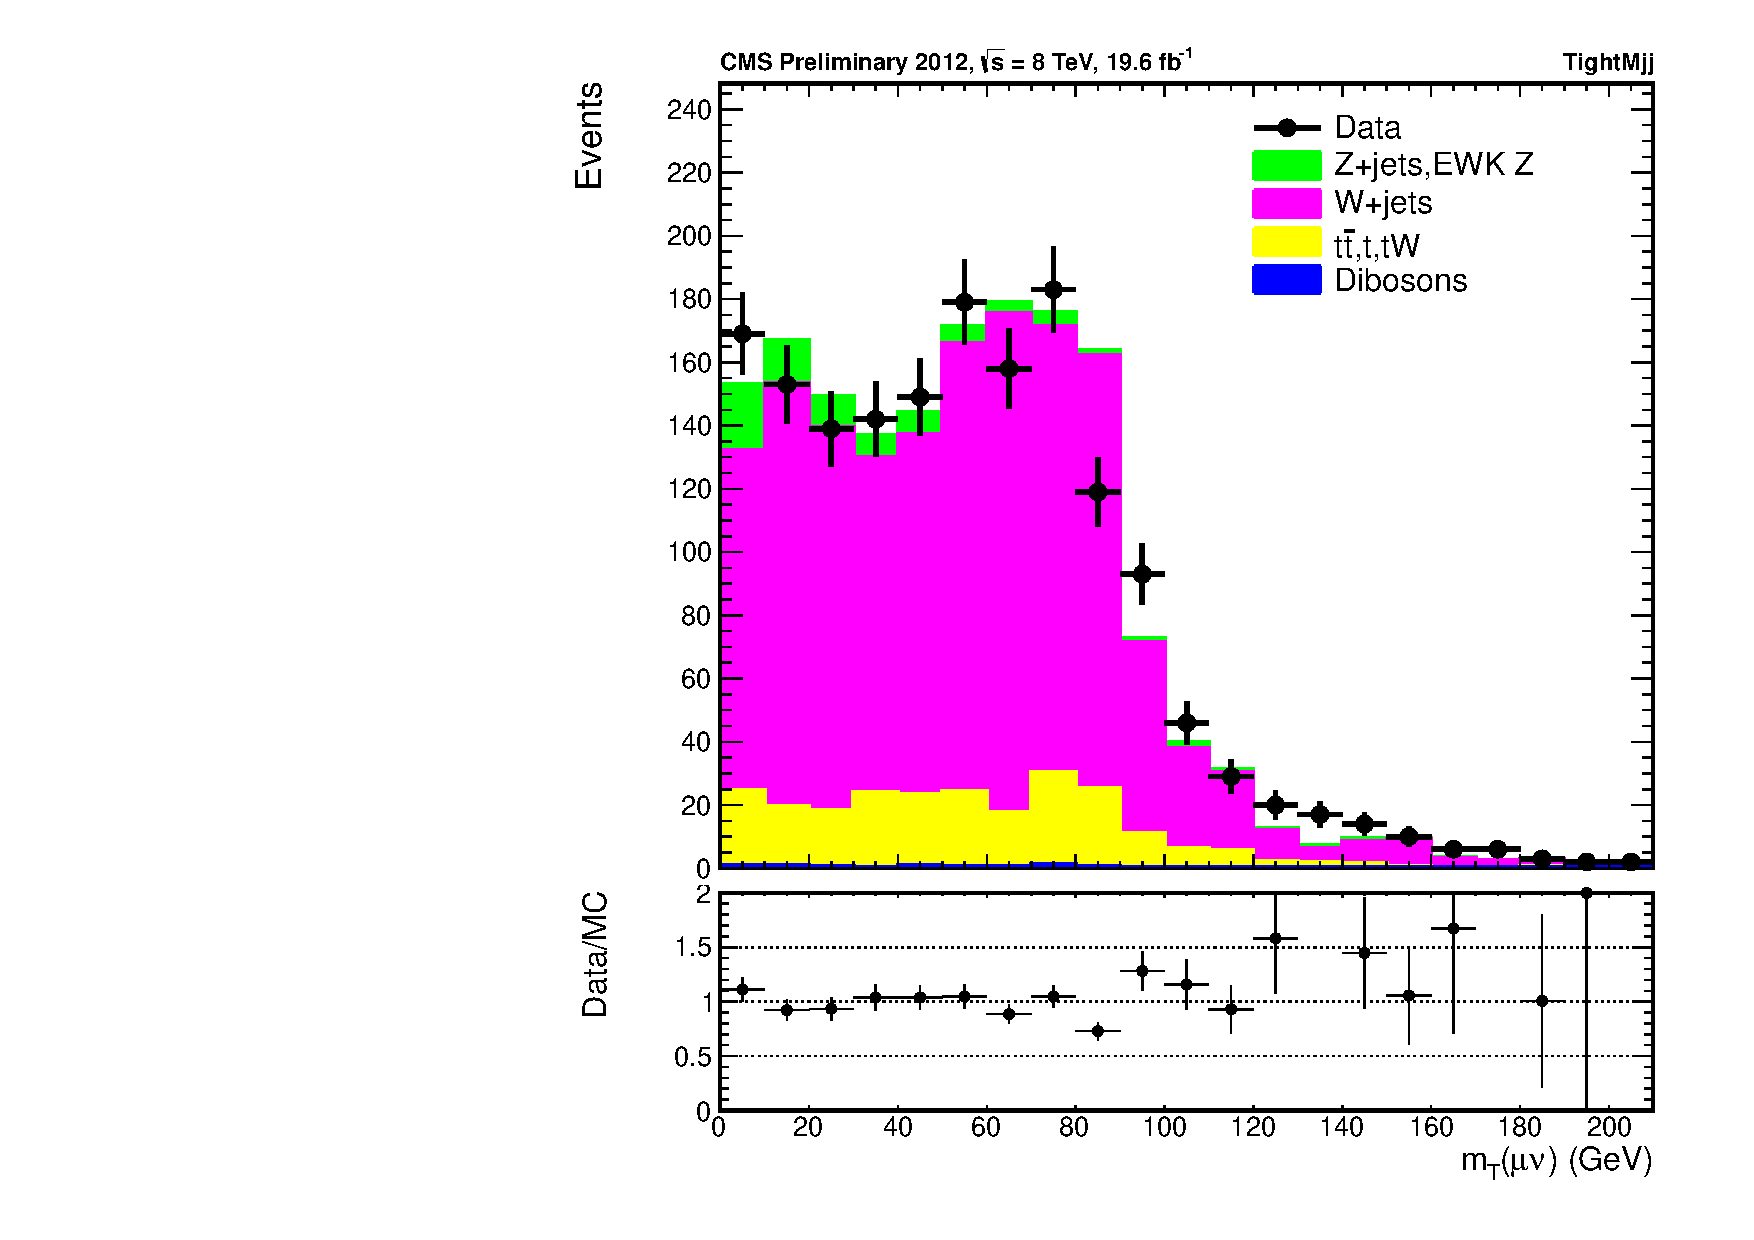
\includegraphics[width=\textwidth]{TalkPics/mt_munu_TightMjj.pdf}
    \column{.33\textwidth}
    $\tau\nu$
    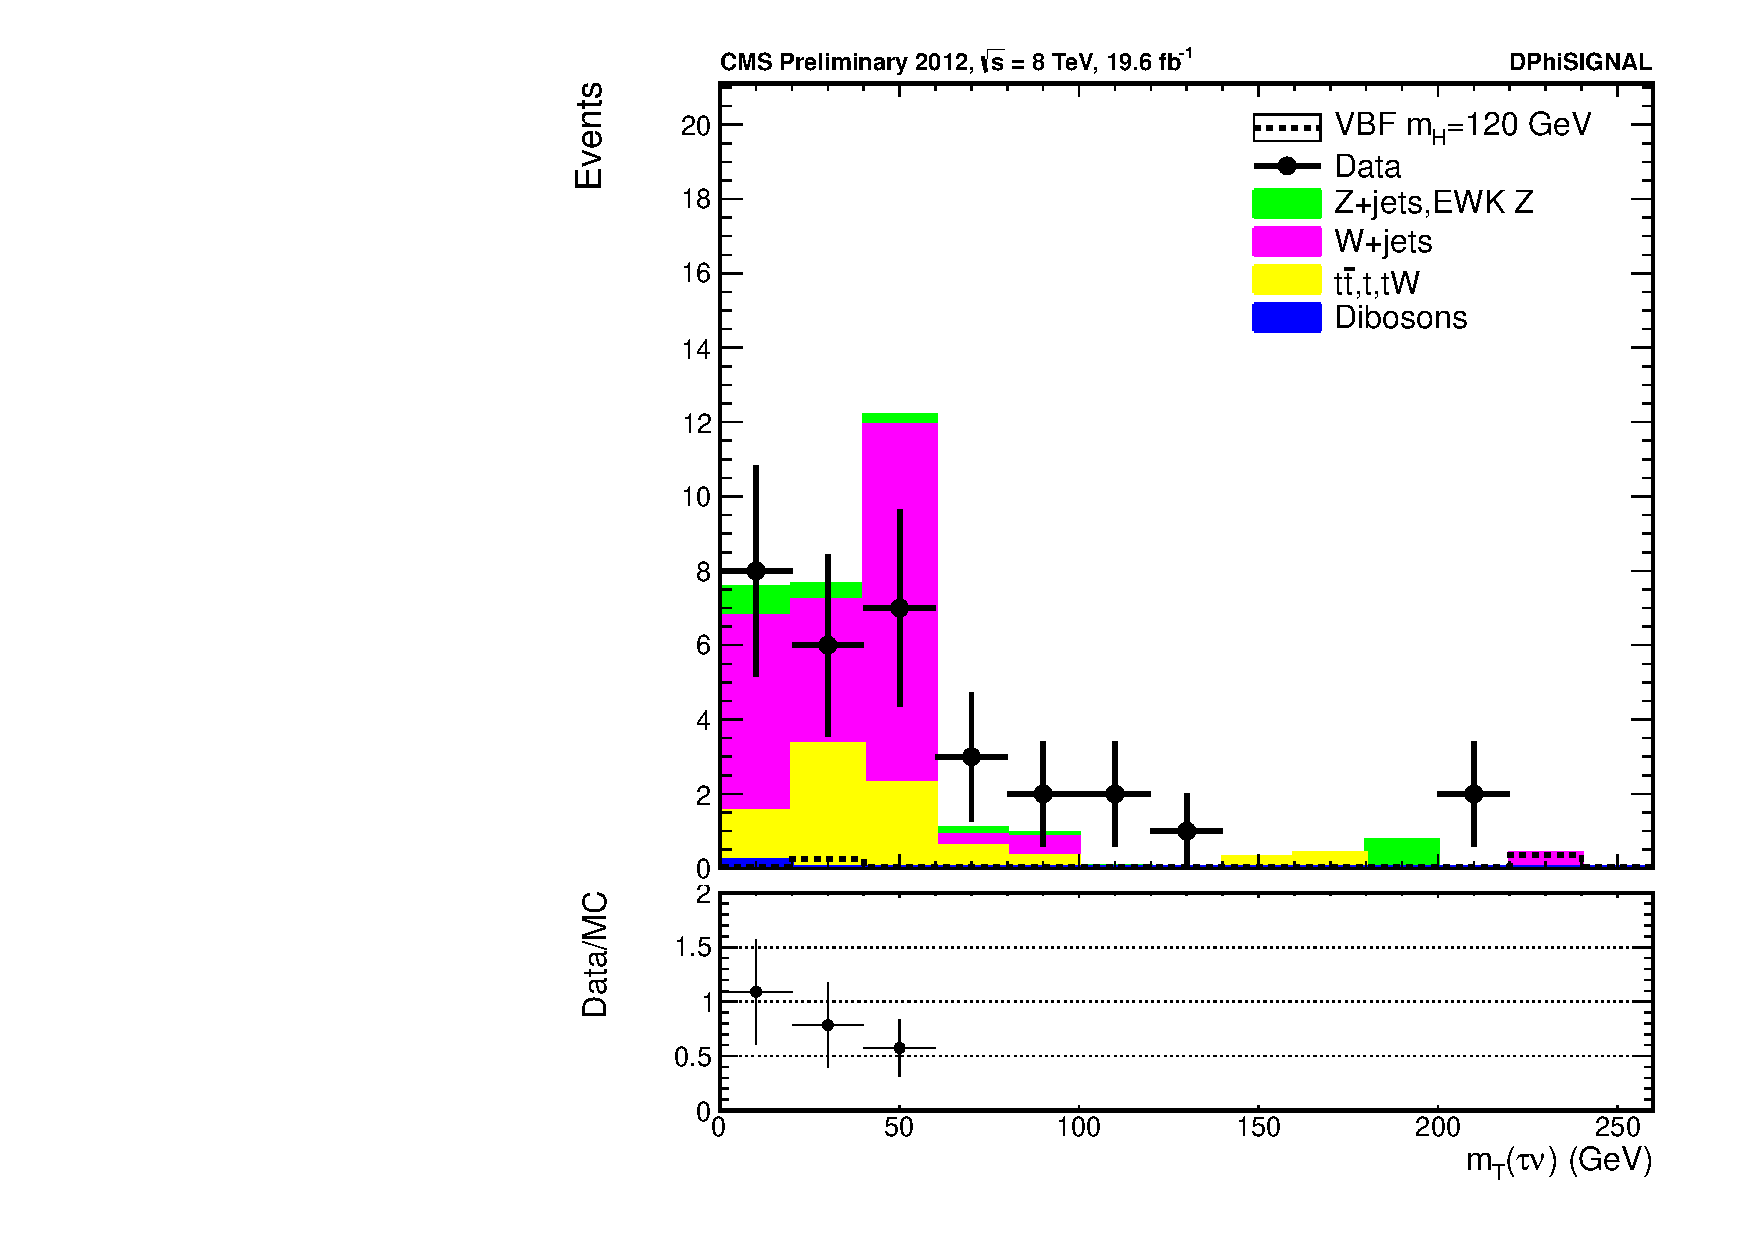
\includegraphics[width=\textwidth]{TalkPics/mt_taunu_2012_DPhiSIGNAL.pdf}
  \end{columns}
\end{frame}
\end{fmffile}
\end{document}
